\documentclass[12pt, a4paper]{article}
\renewcommand{\figurename}{Fig.}

\usepackage[utf8]{inputenc}
\usepackage{amssymb}
\usepackage{anyfontsize}
\usepackage{lipsum}
\usepackage{graphicx}
\usepackage{subcaption}
\usepackage{geometry}
\usepackage{tikz}
\usepackage{array}
\usepackage{enumitem}

%\usepackage[showframe]{geometry}

\usetikzlibrary{automata, positioning, arrows, calc}

\geometry{top      = 2cm,
		  bottom   = 2cm,
		  left     = 2cm,
		  right    = 2cm, 
		  footskip = 1cm}


% ----- STARTING DOCUMENT ----- %

\begin{document}

\pagenumbering{arabic}

\section{Example tiles}

\noindent
In the following, $p$ will be the parameter, $x$ and $y$ will be the clocks, $a$ and $b$ two natural numbers $\in \mathbb{N}$.\\

Tile forcing the following interval: $p \in (\frac{a}{2}, \infty)$.

\begin{figure}[h!]
\begin{center}
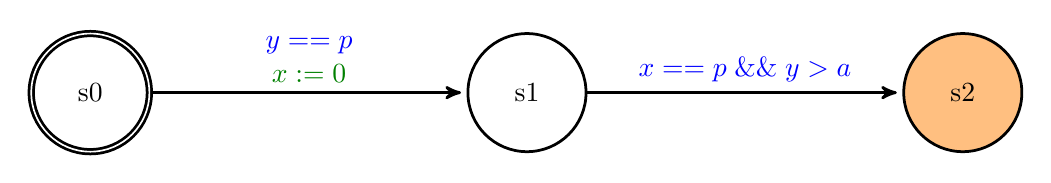
\begin{tikzpicture}
	[->,
	 >=stealth',
	 shorten >=2pt, 
	 auto,
     transform shape, 
     align=center,
     state/.style={thick, circle, draw, minimum size=1.5cm}] 
    
	\node[state, line width = 0.35mm, accepting] (s0) {s0};
	\node[state, right = 4cm of s0, line width = 0.35mm] (s1) {s1}; 
	\node[state, right = 4cm of s1, line width = 0.35mm, fill=orange!50] (s2) {s2}; 
		    
	\draw [line width=0.35mm, auto]
	(s0) edge node{\textcolor{blue}{$y == p$} \\ \textcolor{green!50!black}{$x := 0$}}(s1)
	(s1) edge node{\textcolor{blue}{$x == p \; \&\& \; y > a$}}(s2)
    ;
\end{tikzpicture}
\end{center}
\caption{Tile 2}
\label{tile 2}
\end{figure}


\bigskip

Tile forcing the following interval: $p \in (0, \frac{b}{2})$.

% In node, use accepting for initial states.
% In node, use fill=orange!50 for final states.
% In edge, use \cguard{} for guards.
% In edge, use \creset{} for assignments.

\begin{figure}[h!]
\newcommand{\cguard}{\textcolor{blue}}
\newcommand{\creset}{\textcolor{green!50!black}}

\begin{center}
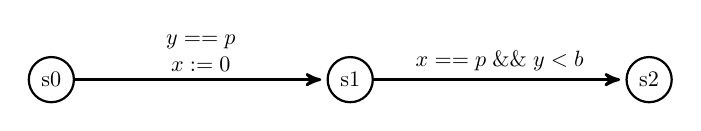
\begin{tikzpicture}[
	->,
	>=stealth',
	shorten >=2pt, 
	auto,
	scale=0.8,
    transform shape, 
    align=center,
    state/.style={thick, circle, draw}
    ] 
    
	\node[state] (s0) {s0};
	\node[state, right = 4cm of s0] (s1) {s1}; 
	\node[state, right = 4cm of s1] (s2) {s2}; 
		    
	\draw [line width=0.35mm]
	(s0) edge node{\cguard{$y == p$} \\ \creset{$x := 0$}}(s1)
	(s1) edge node{\cguard{$x == p \; \&\& \; y < b$}} (s2)
    ;
\end{tikzpicture}
\end{center}

\caption{Tile 2. Forced interval: $p \in (0, \frac{b}{2})$}
\label{tile 2}
\end{figure}



\noindent
The above tiles, namely Tile \ref{tile 1} and Tile \ref{tile 2}, can be considered as the basic building blocks for constructing every other interval, thanks to the possibility of chaining them together, hence restricting the interval in which the parameter $p$ will fall.\\

\noindent
The following one has been obtained by concatenating the aforementioned tiles.\\

Tile forcing the following interval: $p \in (\frac{a}{2}, \frac{b}{2})$.

% In node, use accepting for initial states.
% In node, use fill=orange!50 for final states.
% In edge, use \cguard{} for guards.
% In edge, use \creset{} for assignments.

\begin{figure}[h!]
\newcommand{\cguard}{\textcolor{blue}}
\newcommand{\creset}{\textcolor{green!50!black}}

\begin{center}
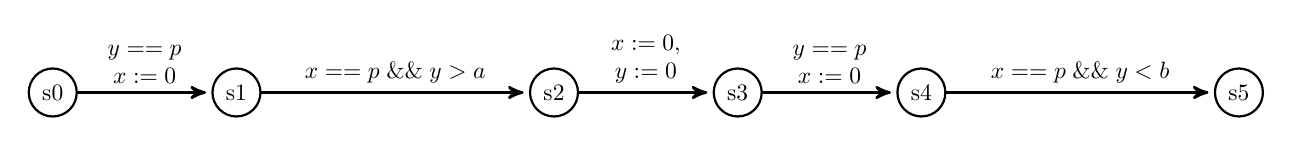
\begin{tikzpicture}[
	->,
	>=stealth',
	shorten >=2pt, 
	auto,
	scale=0.85,
    transform shape, 
    align=center,
    state/.style={thick, circle, draw}
    ] 
    
	\node[state] (s0) {s0};
	\node[state, right = 2cm of s0] (s1) {s1}; 
	\node[state, right = 4cm of s1] (s2) {s2}; 
	\node[state, right = 2cm of s2] (s3) {s3};
	\node[state, right = 2cm of s3] (s4) {s4};
	\node[state, right = 4cm of s4] (s5) {s5};   
		    
	\draw [line width=0.35mm]
	(s0) edge node{\cguard{$y == p$} \\ \creset{$x := 0$}}(s1)
	(s1) edge node{\cguard{$x == p \; \&\& \; y > a$}} (s2)
	(s2) edge node{\creset{$x := 0,$} \\ \creset{$y := 0$}} (s3)
	(s3) edge node{\cguard{$y == p$} \\ \creset{$x := 0$}}(s4)
	(s4) edge node{\cguard{$x == p \; \&\& \; y < b$}} (s5)
    ;
\end{tikzpicture}
\end{center}

\caption{Tile 3}
\label{tile 3}
\end{figure}



\noindent
Please note that Tile \ref{tile 3} can be written more concisely without using concatenation.\\

Tile forcing the following interval: $p \in (\frac{a}{2}, \frac{b}{2})$.

% In node, use accepting for initial states.
% In node, use fill=orange!50 for final states.
% In edge, use \cguard{} for guards.
% In edge, use \creset{} for assignments.

\begin{figure}[h!]
\newcommand{\cguard}{\textcolor{blue}}
\newcommand{\creset}{\textcolor{green!50!black}}

\begin{center}
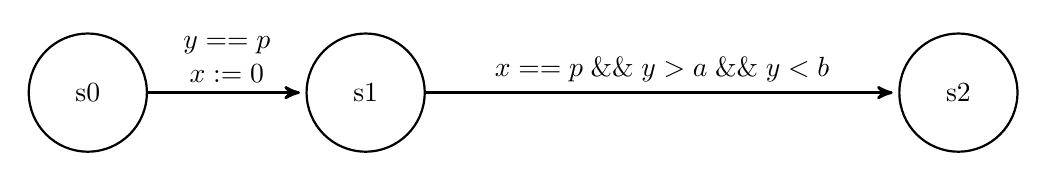
\begin{tikzpicture}[
	->,
	>=stealth',
	shorten >=2pt, 
	auto,
    transform shape, 
    align=center,
    state/.style={thick, circle, draw, minimum size=1.5cm}
    ] 
    
	\node[state] (s0) {s0};
	\node[state, right = 2cm of s0] (s1) {s1}; 
	\node[state, right = 6cm of s1] (s2) {s2};  
		    
	\draw [line width=0.35mm]
	(s0) edge node{\cguard{$y == p$} \\ \creset{$x := 0$}}(s1)
	(s1) edge node{\cguard{$x == p \; \&\& \; y > a \; \&\& \; y < b$}} (s2)
    ;
\end{tikzpicture}
\end{center}

\caption{Tile 4}
\label{tile 4}
\end{figure}



\newpage

\noindent
The following tile has 2 output states, giving rise to the ability of choosing one or the other in an OR condition.\\

Tile forcing the following interval: $p \in (0, \frac{a}{2}) \vee p \in [\frac{b}{2}, \frac{b}{2}]$

% In node, use accepting for initial states.
% In node, use fill=orange!50 for final states.
% In edge, use \cguard{} for guards.
% In edge, use \creset{} for assignments.

\begin{figure}[h!]
\newcommand{\cguard}{\textcolor{blue}}
\newcommand{\creset}{\textcolor{green!50!black}}

\begin{center}
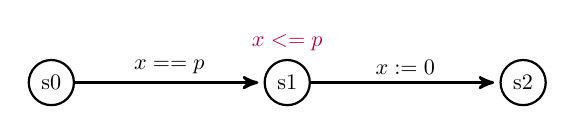
\begin{tikzpicture}[
	->,
	>=stealth',
	shorten >=2pt, 
	auto,
	scale=0.8,
    transform shape, 
    align=center,
    state/.style={thick, circle, draw}
    ] 
    
	\node[state] (s0) {s0};
	\node[state, right = 3cm of s0, label={[text=purple]$x <= p$}] (s1) {s1}; 
	\node[state, right = 3cm of s1] (s2) {s2};

	\draw [line width=0.35mm]
	(s0) edge node{\cguard{$x == p$}} (s1)
	(s1) edge node{\creset{$x := 0$}} (s2)
    ;
\end{tikzpicture}
\end{center}

\caption{Arbitrary interval Tile 5}
\label{arbitrary interval tile 5}
\end{figure}



\noindent
Please note that in such cases, unless some other previous or subsequent tile forces the parameter in a specific interval, our approach is based on trying all the parameter values starting from $n /2$ (or $n / 2 + \alpha$), so the OR tile isn't really non-deterministic in that sense. For example, testing Tile \ref{tile 5} in tChecker with values $a == 8$ and $b == 4$ the result yielded $p == 0.5$.\\

\noindent
The following tile has several inputs and outputs, being the most general type of tile we can build (one with $n$ inputs and $m$ outputs).

% In node, use accepting for initial states.
% In node, use fill=orange!50 for final states.
% In edge, use \cguard{} for guards.
% In edge, use \creset{} for assignments.

\begin{figure}[h!]
\newcommand{\cguard}{\textcolor{blue}}
\newcommand{\creset}{\textcolor{green!50!black}}

\begin{center}
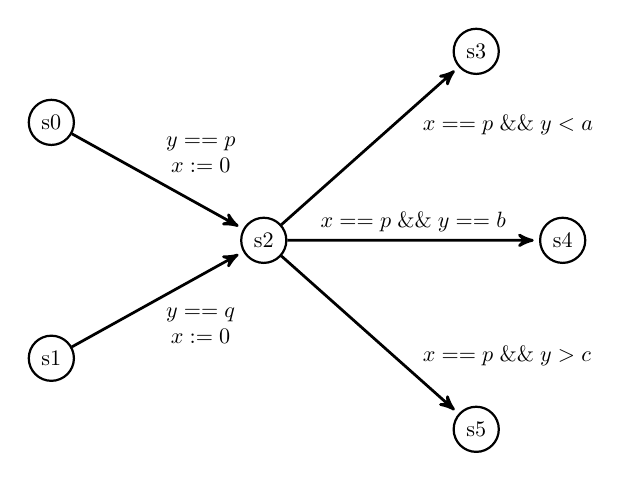
\begin{tikzpicture}[
	->,
	>=stealth',
	shorten >=2pt, 
	auto,
	scale=0.8,,
    transform shape, 
    align=center,
    state/.style={thick, circle, draw}
    ] 
    
	\node[state] (s0) {s0};
	\node[state, below = 3cm of s0] (s1) {s1}; 
	\node[state, right = 3cm of s1] (s2) at ($(s0)!0.5!(s1)$) {s2};
	\node[state, right = 3cm of s2] at ([yshift=3cm]s2) (s3) {s3}; 
	\node[state, right = 4cm of s2] (s4) {s4};
	\node[state, right = 3cm of s2] at ([yshift=-3cm]s2) (s5) {s5}; 

	\draw [line width=0.35mm]
	(s0) edge node{\cguard{$y == p$} \\ \creset{$x := 0$}}(s2)
	(s1) edge node[swap]{\cguard{$y == q$} \\ \creset{$x := 0$}} (s2)
	(s2) edge node[near end, swap]{\cguard{$x == p \; \&\& \; y < a$}} (s3)
	(s2) edge node{\cguard{$x == p \; \&\& \; y == b$}} (s4)
	(s2) edge node[near end]{\cguard{$x == p \; \&\& \; y > c$}} (s5)
    ;
\end{tikzpicture}
\end{center}

\caption{Tile 6}
\label{tile 6}
\end{figure}



\noindent
Understanding whether having multiple input states is useful or not is still under study.

\newpage

\section{Arbitrary intervals}

\noindent
Up to now, we have seen intervals such as these ones: $(0, \frac{b}{2})$ or $(\frac{a}{2}, \frac{b}{2})$, where we can notice a 2 at the denominator of the constants delimiting the interval.\\
One question that may arise is: \emph{Can such intervals be made arbitrarily small?} That is, is it possible to obtain intervals like $(\frac{a}{n}, \frac{b}{n})$, where $n \in \mathbb{N}-\{0\}$ is an arbitrarily-chosen constant?\\
Unfortunately, I don't believe this is actually possible without violating our working assumptions.\\

\noindent
In the following we recap our base assumptions on the TAs we work with:
\begin{enumerate}
\item The grammar for clock constrains does not admit algebraic operations, that is, we cannot have a clock constraint like this: $x < a + b$;
\item TAs are actually nrt-TAs, i.e. a clock cannot be reset and tested in the same transition;
\item We have only two clocks and one parameter (although the constraint on the parameter is not relevant for these considerations).
\end{enumerate}

\noindent
We have to show that it is not possible to construct a tile that is capable of forcing an arbitrarily small interval without violating any of the aforementioned assumptions.\\
For the sake of simplicity with the drawings, we will show it for the case in which $n = 3$, but a generalization of these concepts is straightforward.\\

\noindent
The first case study will try to preserve both nrt and two clocks assumptions. However, this would require illegal clock constraints syntax, as can be seen in the following figure.\\

Tile forcing the following interval: $p \in (0, \frac{a}{3})$.

\begin{figure}[h!]
\begin{center}
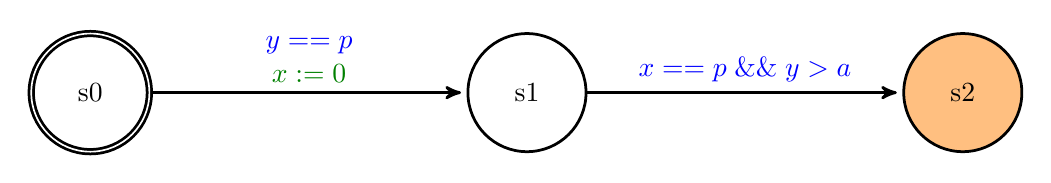
\begin{tikzpicture}
	[->,
	 >=stealth',
	 shorten >=2pt, 
	 auto,
     transform shape, 
     align=center,
     state/.style={thick, circle, draw, minimum size=1.5cm}] 
    
	\node[state, line width = 0.35mm, accepting] (s0) {s0};
	\node[state, right = 4cm of s0, line width = 0.35mm] (s1) {s1}; 
	\node[state, right = 4cm of s1, line width = 0.35mm, fill=orange!50] (s2) {s2}; 
		    
	\draw [line width=0.35mm, auto]
	(s0) edge node{\textcolor{blue}{$y == p$} \\ \textcolor{green!50!black}{$x := 0$}}(s1)
	(s1) edge node{\textcolor{blue}{$x == p \; \&\& \; y > a$}}(s2)
    ;
\end{tikzpicture}
\end{center}
\caption{Tile 2}
\label{tile 2}
\end{figure}


\noindent
Since here we let the first transition fire when y is exactly equal to p, the second transition to fire when y is exactly equal to $2p$ and the last transition to fire when x is exactly equal to $p$ and y less than $a$, since y is never reset, in the last transition it must hold that $y == 3p$. But, since we violated condition (1) above, we cannot use this construction in our analysis.\\

\noindent
Our second case study addresses the nrt nature of the TAs. It is possible to construct arbitrarily small intervals, if we get rid of the nrt property.\\

Tile forcing the following interval: $p \in (0, \frac{a}{3})$.

% In node, use accepting for initial states.
% In node, use fill=orange!50 for final states.
% In edge, use \cguard{} for guards.
% In edge, use \creset{} for assignments.

\begin{figure}[h!]
\newcommand{\cguard}{\textcolor{blue}}
\newcommand{\creset}{\textcolor{green!50!black}}

\begin{center}
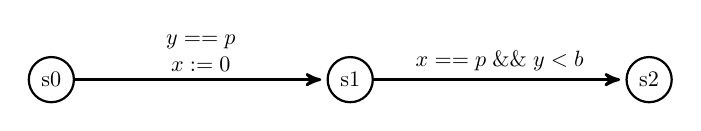
\begin{tikzpicture}[
	->,
	>=stealth',
	shorten >=2pt, 
	auto,
	scale=0.8,
    transform shape, 
    align=center,
    state/.style={thick, circle, draw}
    ] 
    
	\node[state] (s0) {s0};
	\node[state, right = 4cm of s0] (s1) {s1}; 
	\node[state, right = 4cm of s1] (s2) {s2}; 
		    
	\draw [line width=0.35mm]
	(s0) edge node{\cguard{$y == p$} \\ \creset{$x := 0$}}(s1)
	(s1) edge node{\cguard{$x == p \; \&\& \; y < b$}} (s2)
    ;
\end{tikzpicture}
\end{center}

\caption{Tile 2. Forced interval: $p \in (0, \frac{b}{2})$}
\label{tile 2}
\end{figure}



\noindent
Since in this case y is never reset, we can consider x as a sort of counter. At the end, in the last transition y will have a value corresponding to $3p$. The same considerations from the previous case also hold here. But, as mentioned at the beginning, condition (2) is violated, so we cannot use this construction in our analysis.\\

\noindent
The last case affects the number of clocks: we can get a tile forcing an arbitrarily small interval, but at the expense of adding a new clock for each natural $n \in \mathbb{N}-\{0\}$ we want to use as the denominator.\\

Tile forcing the following interval: $p \in (0, \frac{a}{3})$.

% In node, use accepting for initial states.
% In node, use fill=orange!50 for final states.
% In edge, use \cguard{} for guards.
% In edge, use \creset{} for assignments.

\begin{figure}[h!]
\newcommand{\cguard}{\textcolor{blue}}
\newcommand{\creset}{\textcolor{green!50!black}}

\begin{center}
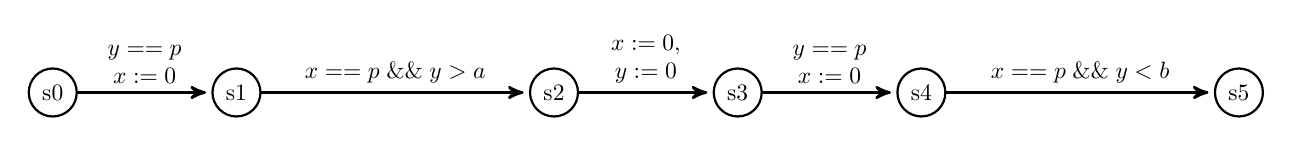
\begin{tikzpicture}[
	->,
	>=stealth',
	shorten >=2pt, 
	auto,
	scale=0.85,
    transform shape, 
    align=center,
    state/.style={thick, circle, draw}
    ] 
    
	\node[state] (s0) {s0};
	\node[state, right = 2cm of s0] (s1) {s1}; 
	\node[state, right = 4cm of s1] (s2) {s2}; 
	\node[state, right = 2cm of s2] (s3) {s3};
	\node[state, right = 2cm of s3] (s4) {s4};
	\node[state, right = 4cm of s4] (s5) {s5};   
		    
	\draw [line width=0.35mm]
	(s0) edge node{\cguard{$y == p$} \\ \creset{$x := 0$}}(s1)
	(s1) edge node{\cguard{$x == p \; \&\& \; y > a$}} (s2)
	(s2) edge node{\creset{$x := 0,$} \\ \creset{$y := 0$}} (s3)
	(s3) edge node{\cguard{$y == p$} \\ \creset{$x := 0$}}(s4)
	(s4) edge node{\cguard{$x == p \; \&\& \; y < b$}} (s5)
    ;
\end{tikzpicture}
\end{center}

\caption{Tile 3}
\label{tile 3}
\end{figure}



\noindent
Similar considerations can be done on why at the end z is equal to $3p$ (it should be trivial to notice at this stage). The tile is nrt, but having more than 2 clocks and thus violating condition (3), we cannot use this construction in our analysis.\\

\noindent
In conclusion of these considerations, it is worth noticing that, in order to construct the aforementioned illegal tiles, the number of states grows linearly with respect to the natural $n \in \mathbb{N}-\{0\}$ we want to use as the denominator: $T(n) = \Theta(n)$.\\
The same growth also happens in the case in which we opt for adding more clocks.\\
Actually, I just figured out it should be possible to obtain the same effect by using only 3 clocks: two of them are required to alternate in setting and testing the parameter (just like the first two in the example violating condition (3)), while the other clock may be used to force the interval like the z clock did in the same example.\\
Hence, attention should be put when combining them for constructing Tiled TAs, due to the growth of the states set and transitions sets (and anything related to this).

\newpage

\section{Arbitrary intervals with nrt tiles}

\noindent
It should be possible to obtain the arbitrary interval restriction while still satisfying assumptions (1), (2) and (3) above by making use of invariants and instantaneous transitions (i.e. transitions that take 0 time units to fire). However, also this construction will not be suitable for our needs, since it violates our hypothesis of time increasing strictly monotonically.\\
For the sake of completeness, we report in the following figures such construction.\\

Tile forcing the following interval: $p \in (0, \frac{a}{k})$, where $k \in \mathbb{N}-\{0\}$ (here it holds $k = 3$).

% In node, use accepting for initial states.
% In node, use fill=orange!50 for final states.
% In edge, use \cguard{} for guards.
% In edge, use \creset{} for assignments.

\begin{figure}[h!]
\newcommand{\cguard}{\textcolor{blue}}
\newcommand{\creset}{\textcolor{green!50!black}}

\begin{center}
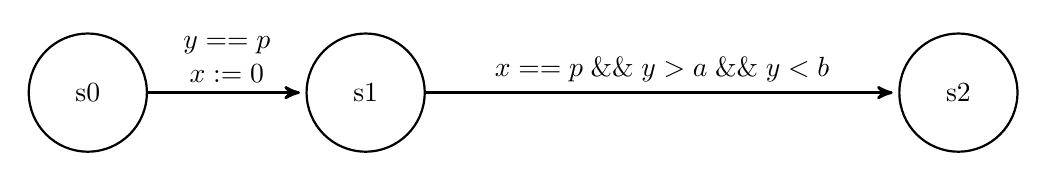
\begin{tikzpicture}[
	->,
	>=stealth',
	shorten >=2pt, 
	auto,
    transform shape, 
    align=center,
    state/.style={thick, circle, draw, minimum size=1.5cm}
    ] 
    
	\node[state] (s0) {s0};
	\node[state, right = 2cm of s0] (s1) {s1}; 
	\node[state, right = 6cm of s1] (s2) {s2};  
		    
	\draw [line width=0.35mm]
	(s0) edge node{\cguard{$y == p$} \\ \creset{$x := 0$}}(s1)
	(s1) edge node{\cguard{$x == p \; \&\& \; y > a \; \&\& \; y < b$}} (s2)
    ;
\end{tikzpicture}
\end{center}

\caption{Tile 4}
\label{tile 4}
\end{figure}



\noindent
As can be seen in the above figure, we can get an arbitrarily small interval by chaining the following sub-tile k times:

% In node, use accepting for initial states.
% In node, use fill=orange!50 for final states.
% In edge, use \cguard{} for guards.
% In edge, use \creset{} for assignments.

\begin{figure}[h!]
\newcommand{\cguard}{\textcolor{blue}}
\newcommand{\creset}{\textcolor{green!50!black}}

\begin{center}
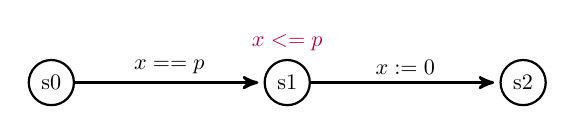
\begin{tikzpicture}[
	->,
	>=stealth',
	shorten >=2pt, 
	auto,
	scale=0.8,
    transform shape, 
    align=center,
    state/.style={thick, circle, draw}
    ] 
    
	\node[state] (s0) {s0};
	\node[state, right = 3cm of s0, label={[text=purple]$x <= p$}] (s1) {s1}; 
	\node[state, right = 3cm of s1] (s2) {s2};

	\draw [line width=0.35mm]
	(s0) edge node{\cguard{$x == p$}} (s1)
	(s1) edge node{\creset{$x := 0$}} (s2)
    ;
\end{tikzpicture}
\end{center}

\caption{Arbitrary interval Tile 5}
\label{arbitrary interval tile 5}
\end{figure}



\noindent
Notice that this ensures that at the end y (which is never reset) will have a value of $y = kp$ and thus the following holds in the last transition: $y = kp < b => p < \frac{b}{k}$, hence implying the interval mentioned above.\\
Also, here we make use of invariants in states to enforce steps every p time units, but this implies a model in which istantaneous transitions are admitted, which is not our case.\\
I have also tried reasoning on obtaining the same result with backward loops, but i fear that in this way we cannot enforce the exact interval we want.

\end{document}
